\documentclass{article}
\usepackage[utf8]{inputenc}
\usepackage[spanish]{babel}
\usepackage[a4paper, total={16cm, 26.5cm}]{geometry}
\usepackage{amsmath}
\usepackage{amsthm}
\usepackage{amssymb}
\usepackage{booktabs}
\usepackage{parskip} 
\usepackage{xcolor}
\usepackage{enumerate}
\usepackage{graphicx}
\title{SOLUCIONES 1ER PARCIAL 2021\vspace{-3em}}
% \author{Nazareno Faillace}
\date{}

\newcommand{\mr}{\mathcal{R}}
\newcommand{\mm}{\mathcal{M}}
\newcommand{\dsum}{\displaystyle\sum}

\begin{document}

\maketitle
% \large{\textbf{}}

\textbf{Ejercicio 1.}

Problema estandarizado para Fase I, considerando $\hat{x}_3=-x_3$:


    \[
    \begin{array}{rrcl}
    \max & \multicolumn{3}{l}{y = -a_1-a_2} \\
    s.a: & x_1+x_2-\hat{x}_3 + a_1 & = & 4 \\
     & 2x_1+\hat{x}_3 + w_1& = & 5 \\
     & 2x_1-x_2 -w_2 + a_2& = & 2 \\
     & x_1,x_2, \hat{x}_3, w_1, w_2,a_1, a_2 & \geq & 0 \\
    \end{array}
    \]

Procedimiento Fase I:

Primera base: $(w_1, a_1, a_2)$, $\bar{b}=(5, 4, 2)$, $y = -6$

Primer pivote: entra $x_1$ a la base, sale $a_2$

Segunda base: $(x_1, w_1, a_1)$, $\bar{b}=(1, 5, 3)$, $y = -3$

Segundo pivote: entra $x_2$ a la base, sale $a_1$

Tercera base: $(x_1, x_2, w_1)$, $\bar{b}=(2, 2, 1)$, $y = 0$

La tercera base es óptima. La base factible inicial del problema es $(x_1, x_2, w_1)$. Al transformar el último diccionario de Fase I en el primer diccionario de Fase II, se ve que $x_3$ tiene costo reducido positivo, por lo tanto la solución no es óptima.

\textbf{Ejercicio 2.}

a) Problema dual:
\[
\begin{array}{rrcl}
\min & \multicolumn{3}{l}{z = -2x_1+8x_2} \\
s.a: & -x_1+x_2 & \geq & 1 \\
 & x_1+x_2 & \geq & 1 \\
 & x_1 & \geq & -2 \\
 & 2x_1+x_2 & \geq & 2 \\
 & y & \geq & 0
\end{array}
\]

b) Óptimo del dual: $y^\ast =(\frac{1}{3}, \frac{4}{3})$

c) Por el teorema visto en la teórica y demostrado en la práctica, el nuevo valor de la función objetivo sería:
\[z^\ast + \frac{1}{2}\cdot\frac{1}{3} + \frac{1}{2}\cdot\frac{4}{3} = 10.833333\dots\]

\textbf{Ejercicio 3.}

a) $\delta \geq -3$

b) $\{(\alpha,\beta)\in\mathbb{R}^2\colon\; \alpha\geq\frac{3}{2}\;\wedge\;\frac{2}{3}\alpha+\beta\leq 2\}$

\textbf{Ejercicio 4.}


\begin{figure}[htpb!]
    \centering
    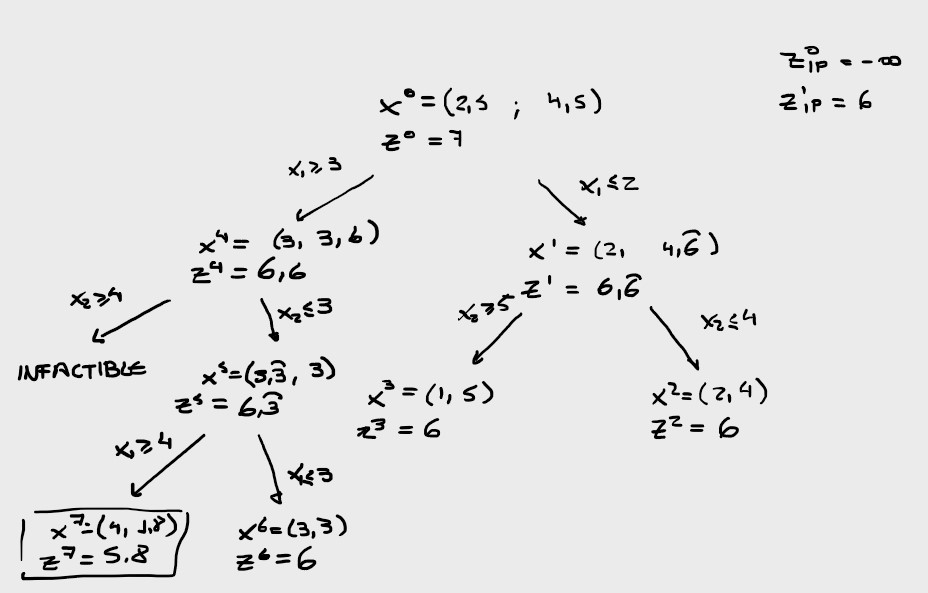
\includegraphics[scale=0.5]{Imagenes/x1.jpg}
    \caption{Empezando con ramificación por $x_1$}
\end{figure}

\begin{figure}[htpb!]
    \centering
    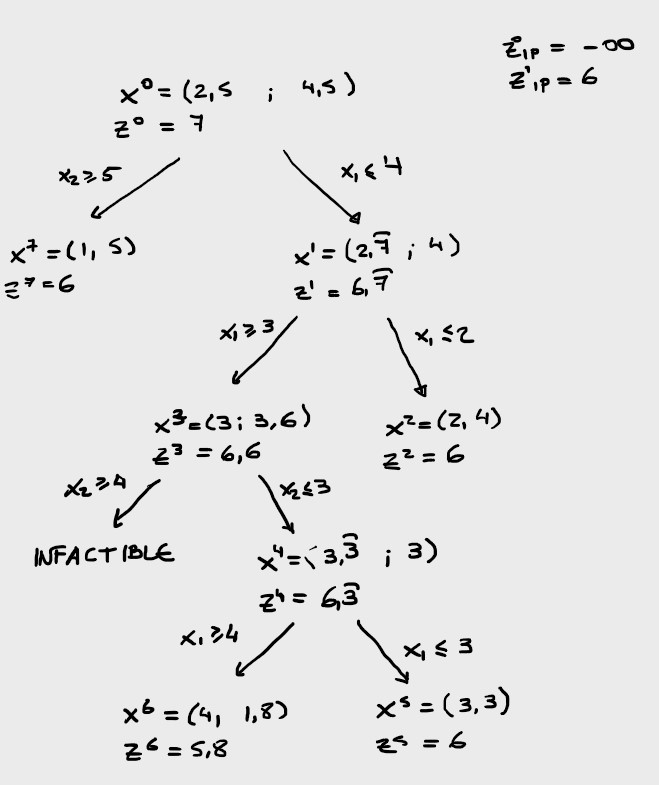
\includegraphics[scale=0.5]{Imagenes/x2.jpg}
    \caption{Empezando con ramificación por $x_2$}
\end{figure}


\end{document}
